\begin{sloppypar}
\subsection*{\textit{\textbf{RQ2: Why can traditional releases deliver addressed issues more quickly?}}}
\end{sloppypar}

\begin{figure}[t!]
	\centering
	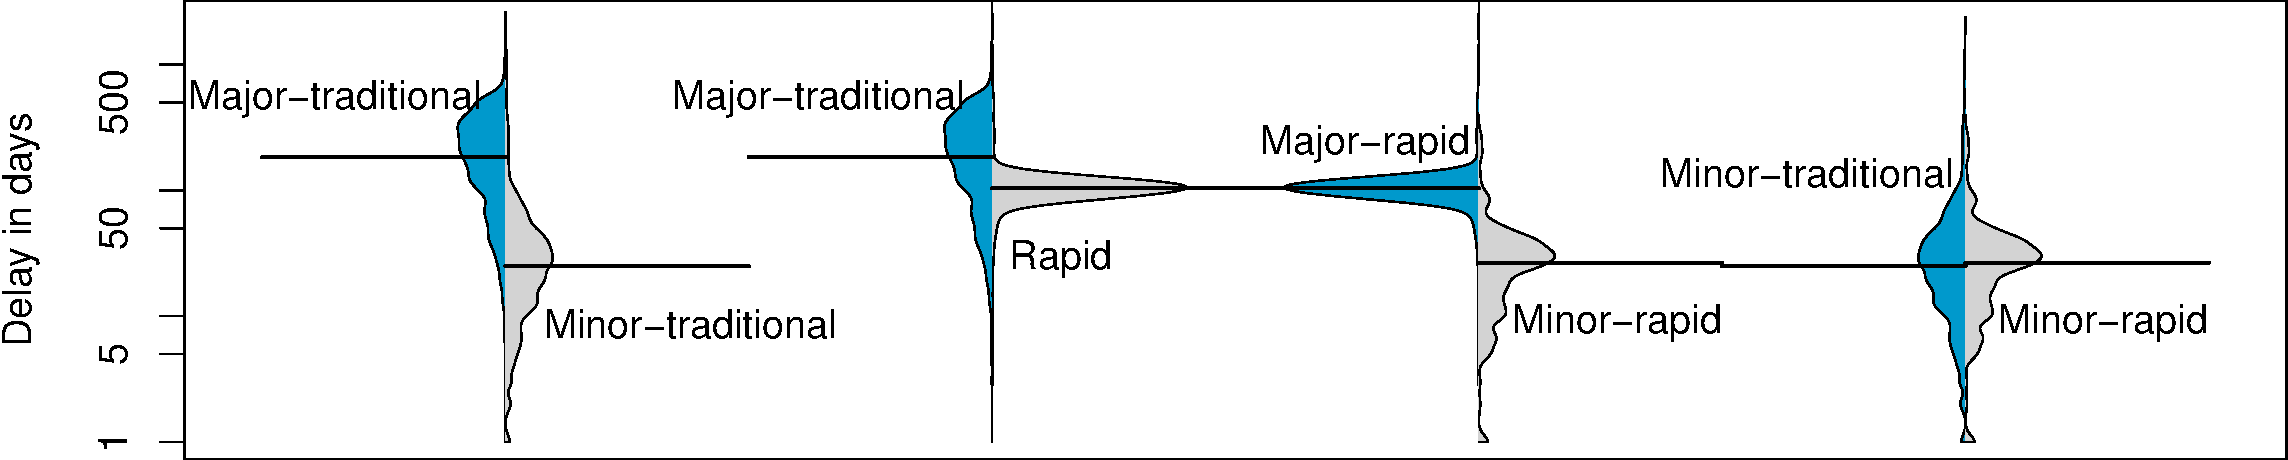
\includegraphics[width=\textwidth,keepaspectratio]
	{chapters/chapter5/figures/rq2/major_vs_minor.pdf}
	\caption{
		Distributions of delivery delay of addressed issues grouped by minor and major
		releases.
	}
	\label{fig:major_vs_minor}
\end{figure}

\begin{sloppypar}
\noindent\textit{\textbf{Observation~3---Minor-traditional releases tend to have
less delivery delay than major/minor-rapid releases.}}\observation{obs:3}
\hyperref[fig:major_vs_minor]{Figure}~\ref{fig:major_vs_minor} shows the distributions of delivery delay
grouped by (1) \textit{major-traditional vs. minor-traditional}, (2)
\textit{major-traditional vs. rapid}, (3) \textit{major-rapid vs. minor-rapid},
and (4) \textit{minor-traditional vs. minor-rapid}. In the comparison of
\textit{major-traditional vs.  minor-traditional}, we observe that
minor-traditional releases are mainly associated with shorter delivery delay.
Furthermore, in the comparison \textit{major-traditional vs. rapid}, rapid
releases deliver addressed issues more quickly than major-traditional releases
on average ($p<2.2e^{-16}$ with a $medium$ effect-size, \ie  $delta=0.40$). 
\end{sloppypar}

The Firefox rapid release cycle includes ESR releases (see
\hyperref[ch:background]{Chapter}~\ref{ch:background}) and a few minor
stabilization and security releases. These releases also deliver addressed
issues more quickly than major-rapid releases (\textit{major-rapid vs.
minor-rapid}) with a $p<2.2e^{-16}$ and a $large$ effect-size, \ie $delta=0.92$.
Furthermore, we do not observe a statistically significant difference between
distributions in the comparison of \textit{minor-traditional vs. minor-rapid}
($p=0.68$).

Minor-traditional releases have the lowest delivery delay (median of 25
days). This is likely because they are more focused on a particular set of
issues that, once addressed, should be released immediately. For example, the
release history documentation of Firefox shows that minor releases are usually
related to stability and security
issues.\footnote{\url{https://www.mozilla.org/en-US/firefox/releases/}}\\

\begin{figure}[t!]
	\centering
	\subfloat[Only Major]{           
		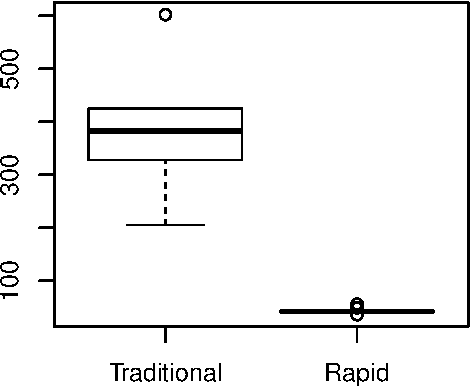
\includegraphics[width=0.45\columnwidth,keepaspectratio]
		{chapters/chapter5/figures/releases/majorreleases_length.pdf}
		\label{fig:majorreleases_length}
	}
	\subfloat[Major and Minor]{
		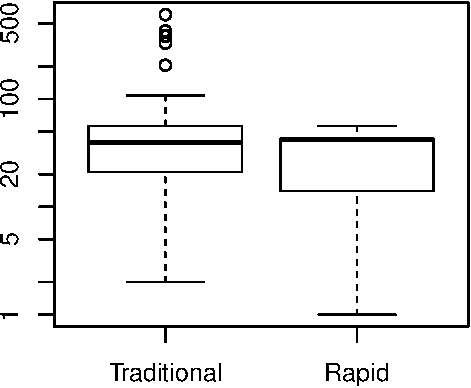
\includegraphics[width=0.45\columnwidth,keepaspectratio]
		{chapters/chapter5/figures/releases/releases_length.pdf}
		\label{fig:releases_length}
	}
	\caption{Release frequency (in days). The outliers in figure~(b)
		represent the major-traditional releases.}
	\label{fig:release_length_analysis}
\end{figure}

\noindent\textit{\textbf{Observation~4---When considering both
minor and major releases, the time span between traditional and rapid releases
are roughly the same.}}\observation{obs:4}
Since we observe that delivery delay is shorter on average in traditional
releases, we also investigate the length of the release cycles to better
understand our previous results (see \hyperref[obs:2]{Observation}~\ref{obs:2}).
\hyperref[fig:majorreleases_length]{Figure}~\ref{fig:majorreleases_length} shows that, at first glance, one may
speculate that rapid releases should deliver addressed issues more quickly
because releases are produced more frequently.  However, if we consider both
major and minor releases---as shown in \hyperref[fig:releases_length]{Figure}~\ref{fig:releases_length}---we
observe that both release strategies deliver releases at roughly the same rate
on average (median of $40$ and $42$ days for traditional and rapid releases,
respectively).\\

\conclusionbox{
Minor-traditional releases are one of the main reasons why the traditional
release strategy can deliver addressed issues more quickly than the rapid
release strategy. Furthermore, the lengths of the release cycles are roughly the
same between traditional and rapid releases when both minor and major releases
are considered.
}

